\documentclass{scrartcl}

\usepackage{siunitx}
\usepackage{graphicx}
\usepackage{caption}
\usepackage{glossaries}
\usepackage[english]{babel}
\usepackage{booktabs}
\usepackage[linktoc=all,hidelinks]{hyperref}
\usepackage{fontspec}
% \usepackage{authblk}
\usepackage{unicode-math}

% \makeatletter
% \renewcommand\AB@affilsepx{,~ \protect\Affilfont}
% \makeatother

\setkomafont{author}{\sffamily}

\newcommand{\nump}[2]{\num[round-mode=places,round-precision=#2]{#1}}
\DeclareGraphicsExtensions{.pdf,.eps}
\bibliographystyle{unsrt}

\title{Report}
\subtitle{A study of machine learning algorithms for reconstruction of missing energy in particle physics experiments.}
% \subject{Statistical Machine Learning}

\author{
  Max Isacson, \url{max.isacson@physics.uu.se}
  \and
  Mikael M\aa rtensson, \url{mikael.martensson@physics.uu.se}
  \and
  Camila Rangel Smith, \url{camila.rangel@physics.uu.se}
  \and
  Henrik Öhman, \url{ohman@cern.ch}
}
% \author[1]{Max Isacsson}
% \author[2]{Mikael M\aa rtensson}
% \author[3]{Camila Rangel Smith}
% \author[4]{Henrik \"{O}hman}
% \affil[1]{\small\url{max.isacsson@physics.uu.se}}
% \affil[2]{\url{mikael.martensson@physics.uu.se}}
% \affil[3]{\url{camila.rangel@physics.uu.se}}
% \affil[4]{\url{ohman@cern.ch}}

\newacronym{NN}{NN}{Neural Network}

\newcommand{\etmiss}{$E_\mathrm{T}^\text{miss}$}
\newcommand{\exmiss}{$E_x^\text{miss}$}
\newcommand{\eymiss}{$E_y^\text{miss}$}

\begin{document}
\maketitle

% \begin{figure}
%     \centering
%     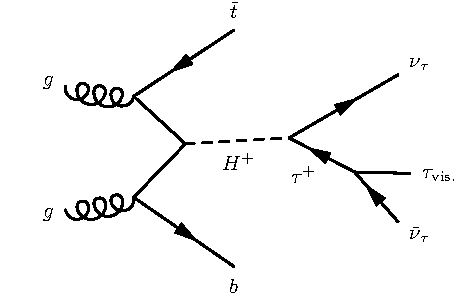
\includegraphics[width=.7\textwidth]{fig/heavyHplustaunu4fs.pdf}
%     \caption{Feynman diagram of the production and decay of a charged Higgs boson. Not shown is the hadronic top decay $\bar t \to \bar b W^-(q \bar q')$.}\label{fig:hplus}
% \end{figure}

\section{Introduction}

\section{The Dataset}
\subsection{Structure}
The dataset consists of simulated $pp$ collision events, in which a charged Higgs is produced and decays as $H^+\to\tau\nu$. Each event is described by one set of observable variables and one set of unobservable variables.

Observable variables:
\begin{itemize}
    \item \exmiss, \eymiss --- The $x$- and $y$-components of the missing energy.
    \item $P_{\tau_\mathrm{vis.}}$ --- The 4-momentum of the visible (hadronic) part of the $\tau$ decay.
    \item $P_{b_0}$, $P_{b_1}$, $P_{q_0}$, $P_{q_1}$ --- The 4-momenta of the two $b$-jets and two light jets.
\end{itemize}

Unobservable variables:
\begin{itemize}
    \item $P_{\nu_\tau}$ --- The 4-momentum of the neutrino from the charged Higgs decay.
    \item $P_{\bar\nu_\tau}$ --- The 4-momentum of the neutrino from the $\tau$ decay.
\end{itemize}

\subsection{Production}
MG5\_aMC@NLO \cite{Alwall:2014hca} is used for the matrix element computation of $gg / q \bar q \to H^+$ and the event simulation. The events are then passed to PYTHIA8 \cite{Sjöstrand2015159} for the showering and hadronization, and for the $H^+\to \tau\nu$ decay. Finally, the detector response is simulated using DELPHES \cite{Favereau2014} with an ATLAS-like geometry.

\subsection{Estimated and true quantities}
The true quantities for both the observable and the unobservable variables are available as output from the event simulation. The estimated values for the observable variables are reconstructed from the output from the detector response simulation.

\section{Solution method}

\subsection{Predictor selection}

\subsection{Neural Network}

The data needs to be scaled to avoid the tails of the neural network activation functions and improve the learning rate. The method used here is to scale it such that the minimum is -1 and the maximum is 1 for each training set variable. The test set data is scaled using the scaling parameters computed from the training set. Another scaling method would be to scale the mean to 0 and the standard deviation to 1, but this was found to slow down the training and give worst result.

The neural network implemented here uses Python with SciPy \cite{scipy}, Numpy \cite{numpy}, and Pandas \cite{pandas} for general data processing, and Keras \cite{keras} for the actual neural network. The number of input nodes is restricted to the 19 selected predictor variables and the output to the target dimension of 1. Since the network is used for regression, the activation functions between the last hidden layer and the output must be linear.

Training is performed using stochastic gradient descent with the Nesterov method \cite{nesterov} and a mean-squared-error loss function. The learning rate was set to 0.1, the learning rate decay to $\num{1e-6}$, and the momentum to 0.9.

A large number of configurations of the hidden layers were tested by varying the number of layers, the number of perceptrons in each layer, and the activation functions (sigmoid, tanh, and softmax). Sigmoid activation functions produced the best result for a fixed training period. A network with two hidden layers (i.e. 4 layers counting the 19 node input layer and 1 node output layer) with 25 and 10 perceptrons was found to be sufficiently complex. Using deeper networks, e.g. one with 4 hidden layer with 20, 35, 25, and 15 perceptrons, did not improve the result.


\section{Results}

\section{Discussion}

% Mention that we use phi(met) when calculating the mT for the prediction. In principle we should predict phi as well. 

\bibliography{refs}

\end{document}
